\begin{figure}[h!p]
\begin{framed}
  Step 0 (optional): infer a graph
  \begin{center}
    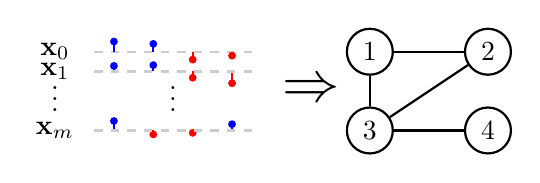
\begin{tikzpicture}[thick]
      \node at (0,0) {$\mathbf{x}_0$};
      \path[black!20!white, dashed]
      (0.5,0) edge (2.5,0);
      \path
      (0.75, 0) edge[blue] (0.75, 0.13)
      (1.25, 0) edge[blue] (1.25, 0.1)
      (1.75, 0) edge[red] (1.75, -0.1)
      (2.25, 0) edge[red] (2.25, -0.05);
      \node[fill, circle, inner sep = 1pt, blue] at (0.75, 0.13) {};
      \node[fill, circle, inner sep = 1pt, blue] at (1.25, 0.1) {};
      \node[fill, circle, inner sep = 1pt, red] at (1.75, -0.1) {};
      \node[fill, circle, inner sep = 1pt, red] at (2.25, -0.05) {};
      \node at (0,-0.25) {$\mathbf{x}_1$};
      \begin{scope}[yshift=-0.25cm]
        \path
        (0.75, 0) edge[blue] (0.75, 0.07)
        (1.25, 0) edge[blue] (1.25, 0.08)
        (1.75, 0) edge[red] (1.75, -0.08)
        (2.25, 0) edge[red] (2.25, -0.15);
        \node[fill, circle, inner sep = 1pt,blue] at (0.75, 0.07){};
        \node[fill, circle, inner sep = 1pt,blue] at (1.25, 0.08){};
        \node[fill, circle, inner sep = 1pt,red] at (1.75, -0.08){};
        \node[fill, circle, inner sep = 1pt,red] at (2.25, -0.15){};        
      \end{scope}

      \path[black!20!white, dashed]
      (0.5,-0.25) edge (2.5,-0.25);
      \node at (0,-0.5) {\vdots};
      \node at (0,-1) {$\mathbf{x}_m$};
      \begin{scope}[yshift=-1cm]
        \path
        (0.75, 0) edge[blue] (0.75, 0.12)
        (1.25, 0) edge[red] (1.25, -0.05)
        (1.75, 0) edge[red] (1.75, -0.03)
        (2.25, 0) edge[blue] (2.25, 0.08);
        \node[fill, circle, inner sep = 1pt, blue] at (0.75, 0.12){};
        \node[fill, circle, inner sep = 1pt, red] at (1.25, -0.05){};
        \node[fill, circle, inner sep = 1pt, red] at (1.75, -0.03){};
        \node[fill, circle, inner sep = 1pt, blue] at (2.25, 0.08){};        
      \end{scope}
      \node at (1.5,-0.5) {\vdots};
      \path[black!20!white, dashed]
      (0.5,-1) edge (2.5,-1);

      \node at (3.25, -0.5) {\huge{$\Rightarrow$}};

      \begin{scope}[xshift=4cm]
        \node[draw, circle](a) at (0,0) {1};
        \node[draw, circle](b) at (1.5,0) {2};
        \node[draw, circle](c) at (1.5,-1) {4};
        \node[draw, circle](d) at (0,-1) {3};
      \end{scope}
      \path
      (a) edge (b)
      edge (d)
      (b) edge (d)
      (c) edge (d);
    \end{tikzpicture}
  \end{center}
  
  Step 1: infer translations (Subsection B)
  \begin{center}
    \begin{tikzpicture}[thick]      
      \begin{scope}[xshift=0cm]
        \node[draw, circle](a) at (0,0) {1};
        \node[draw, circle](b) at (1.5,0) {2};
        \node[draw, circle](c) at (1.5,-1) {4};
        \node[draw, circle](d) at (0,-1) {3};
      \end{scope}
      \path
      (a) edge (b)
      edge (d)
      (b) edge (d)
      (c) edge (d);
      \node at (2.75, -0.5) {\huge{$\Rightarrow$}};
      \begin{scope}[xshift=4cm, scale=0.5, yshift=0.5cm]
        \node[draw, inner sep=2pt, circle](a) at (0,0) {};
        \node[draw, inner sep=2pt, circle](b) at (1.5,0) {};
        \node[draw, inner sep=2pt, circle](c) at (1.5,-1) {};
        \node[draw, inner sep=2pt, circle](d) at (0,-1) {};
      \end{scope}
      \path[black!20!white]
      (a) edge (b)
      edge (d)
      (b) edge (d)
      (c) edge (d);
      \path[->,>=stealth']
      (a) edge (b)      
      (d) edge (c);
      \begin{scope}[xshift=4cm, scale=0.5, yshift=-1.5cm]
        \node[draw, inner sep=2pt, circle](a) at (0,0) {};
        \node[draw, inner sep=2pt, circle](b) at (1.5,0) {};
        \node[draw, inner sep=2pt, circle](c) at (1.5,-1) {};
        \node[draw, inner sep=2pt, circle](d) at (0,-1) {};
      \end{scope}
      \path[black!20!white]
      (a) edge (b)
      edge (d)
      (b) edge (d)
      (c) edge (d);
      \path[->,>=stealth']
      (b) edge (a)      
      (c) edge (d);
      \begin{scope}[xshift=5.5cm, scale=0.5, yshift=0.5cm]
        \node[draw, inner sep=2pt, circle](a) at (0,0) {};
        \node[draw, inner sep=2pt, circle](b) at (1.5,0) {};
        \node[draw, inner sep=2pt, circle](c) at (1.5,-1) {};
        \node[draw, inner sep=2pt, circle](d) at (0,-1) {};
      \end{scope}
      \path[black!20!white]
      (a) edge (b)
      edge (d)
      (b) edge (d)
      (c) edge (d);
      \path[->,>=stealth']
      (a) edge (d);
      \begin{scope}[xshift=5.5cm, scale=0.5, yshift=-1.5cm]
        \node[draw, inner sep=2pt, circle](a) at (0,0) {};
        \node[draw, inner sep=2pt, circle](b) at (1.5,0) {};
        \node[draw, inner sep=2pt, circle](c) at (1.5,-1) {};
        \node[draw, inner sep=2pt, circle](d) at (0,-1) {};
      \end{scope}
      \path[black!20!white]
      (a) edge (b)
      edge (d)
      (b) edge (d)
      (c) edge (d);
      \path[->,>=stealth']
      (d) edge (a);
    \end{tikzpicture}
  
  \end{center}
  
  Step 2: design convolution weight-sharing (Subsection C)

  \begin{center}
    \begin{tikzpicture}[thick]      
      \begin{scope}[xshift=0cm, scale=0.75, yshift=0.5cm]
        \node[inner sep=2pt](w) at (-1.0,-0.5) {$w_1 \times$};
        \node[draw, inner sep=2pt, circle](a) at (0,0) {};
        \node[draw, inner sep=2pt, circle](b) at (1.5,0) {};
        \node[draw, inner sep=2pt, circle](c) at (1.5,-1) {};
        \node[draw, inner sep=2pt, circle](d) at (0,-1) {};       
      \end{scope}
      \path[black!20!white]
      (a) edge (b)
      edge (d)
      (b) edge (d)
      (c) edge (d);
      \path[->,>=stealth']
      (a) edge (b)      
      (d) edge (c);
      \begin{scope}[xshift=0cm, scale=0.75, yshift=-1.5cm]
        \node[inner sep=2pt](w) at (-1.0,-0.5) {+ $w_2 \times$};
        \node[draw, inner sep=2pt, circle](a) at (0,0) {};
        \node[draw, inner sep=2pt, circle](b) at (1.5,0) {};
        \node[draw, inner sep=2pt, circle](c) at (1.5,-1) {};
        \node[draw, inner sep=2pt, circle](d) at (0,-1) {};
      \end{scope}
      \path[black!20!white]
      (a) edge (b)
      edge (d)
      (b) edge (d)
      (c) edge (d);
      \path[->,>=stealth']
      (b) edge (a)      
      (c) edge (d);
      \begin{scope}[xshift=2.5cm, scale=0.75, yshift=0.5cm]
        \node[inner sep=2pt](w) at (-1.0,-0.5) {+ $w_3 \times$};
        \node[draw, inner sep=2pt, circle](a) at (0,0) {};
        \node[draw, inner sep=2pt, circle](b) at (1.5,0) {};
        \node[draw, inner sep=2pt, circle](c) at (1.5,-1) {};
        \node[draw, inner sep=2pt, circle](d) at (0,-1) {};
      \end{scope}
      \path[black!20!white]
      (a) edge (b)
      edge (d)
      (b) edge (d)
      (c) edge (d);
      \path[->,>=stealth']
      (a) edge (d);
      \begin{scope}[xshift=2.5cm, scale=0.75, yshift=-1.5cm]
        \node[inner sep=2pt](w) at (-1.0,-0.5) {+ $w_4 \times$};      
        \node[draw, inner sep=2pt, circle](a) at (0,0) {};
        \node[draw, inner sep=2pt, circle](b) at (1.5,0) {};
        \node[draw, inner sep=2pt, circle](c) at (1.5,-1) {};
        \node[draw, inner sep=2pt, circle](d) at (0,-1) {};
      \end{scope}
      \path[black!20!white]
      (a) edge (b)
      edge (d)
      (b) edge (d)
      (c) edge (d);
      \path[->,>=stealth']
      (d) edge (a);

      \begin{scope}[xshift=5.0cm, scale=0.75, yshift=-0.5cm]
        \node[inner sep=2pt](w) at (-1.0,-0.5) {+ $w_0 \times$};
        \node[draw, inner sep=2pt, circle](a) at (0,0) {};
        \node[draw, inner sep=2pt, circle](b) at (1.5,0) {};
        \node[draw, inner sep=2pt, circle](c) at (1.5,-1) {};
        \node[draw, inner sep=2pt, circle](d) at (0,-1) {};
      \end{scope}
      \path[black!20!white]
      (a) edge (b)
      edge (d)
      (b) edge (d)
      (c) edge (d);
      \path[]
      (a) edge [loop above] (a)
      (b) edge [loop above] (b)
      (c) edge [loop below] (c)
      (d) edge [loop below] (d);

    \end{tikzpicture}
  
  \end{center}
  
  Step 3: design data-augmentation (Subsection D)
  \begin{center}
    \begin{tikzpicture}[thick]      
      \begin{scope}[xshift=0cm]
        \node[draw, inner sep = 2pt, circle](a) at (0,0) {};
        \node[draw, inner sep = 2pt, circle](b) at (1.5,0) {};
        \node[draw, inner sep = 2pt, circle](c) at (1.5,-1) {};
        \node[draw, inner sep = 2pt, circle](d) at (0,-1) {};
        \path[]
        (0, 0) edge[blue] (0, 0.52)
        (1.5, 0) edge[blue] (1.5, 0.4)
        (0, -1) edge[red] (0, -1.4)
        (1.5, -1) edge[red] (1.5, -1.2);
        \node[fill, circle, inner sep = 1pt, blue] at (0, 0.52) {};
        \node[fill, circle, inner sep = 1pt, blue] at (1.5, 0.4) {};
        \node[fill, circle, inner sep = 1pt, red] at (0, -1.4) {};
        \node[fill, circle, inner sep = 1pt, red] at (1.5, -1.2) {};
      \end{scope}
      \node at (-0.5,-0.5) {$\mathbf{x}_0$};
      \path[black!20!white]
      (a) edge (b)
      edge (d)
      (b) edge (d)
      (c) edge (d);
      \node at (2.25, -0.5) {\huge{$\Rightarrow$}};
      \begin{scope}[xshift=3cm, scale=0.5, yshift=0.75cm]
        \node[draw, inner sep=2pt, circle](a) at (0,0) {};
        \node[draw, inner sep=2pt, circle](b) at (1.5,0) {};
        \node[draw, inner sep=2pt, circle](c) at (1.5,-1) {};
        \node[draw, inner sep=2pt, circle](d) at (0,-1) {};
      \end{scope}
      \path[black!20!white]
      (a) edge (b)
      edge (d)
      (b) edge (d)
      (c) edge (d);
      \path[->,>=stealth']
      (a) edge (b)      
      (d) edge (c);
      \begin{scope}[xshift=4.5cm, scale=0.5, yshift = 0.75cm]
        \node[draw, inner sep = 2pt, circle](a) at (0,0) {};
        \node[draw, inner sep = 2pt, circle](b) at (1.5,0) {};
        \node[draw, inner sep = 2pt, circle](c) at (1.5,-1) {};
        \node[draw, inner sep = 2pt, circle](d) at (0,-1) {};
        \path[]
        (1.5, 0) edge[blue] (1.5, 0.52)
        %% (1.5, 0) edge[blue] (1.5, 0.4)
        (1.5, -1) edge[red] (1.5, -1.4);
        %% (1.5, -1) edge[red] (1.5, -1.2);
        \node[fill, circle, inner sep = 1pt, blue] at (1.5, 0.52) {};
        %% \node[fill, circle, inner sep = 1pt, blue] at (1.5, 0.4);
        \node[fill, circle, inner sep = 1pt, red] at (1.5, -1.4) {};
        %% \node[fill, circle, inner sep = 1pt, red] at (1.5, -1.2);
        \path[black!20!white]
      (a) edge (b)
      edge (d)
      (b) edge (d)
      (c) edge (d);
      \end{scope}      
      \begin{scope}[xshift=3cm, scale=0.5, yshift=-1.75cm]
        \node[draw, inner sep=2pt, circle](a) at (0,0) {};
        \node[draw, inner sep=2pt, circle](b) at (1.5,0) {};
        \node[draw, inner sep=2pt, circle](c) at (1.5,-1) {};
        \node[draw, inner sep=2pt, circle](d) at (0,-1) {};
      \end{scope}
      \path[black!20!white]
      (a) edge (b)
      edge (d)
      (b) edge (d)
      (c) edge (d);
      \path[->,>=stealth']
      (b) edge (a)      
      (c) edge (d);
      \begin{scope}[xshift=4.5cm, scale=0.5, yshift=-1.75cm]
        \node[draw, inner sep = 2pt, circle](a) at (0,0) {};
        \node[draw, inner sep = 2pt, circle](b) at (1.5,0) {};
        \node[draw, inner sep = 2pt, circle](c) at (1.5,-1) {};
        \node[draw, inner sep = 2pt, circle](d) at (0,-1) {};
        \path[]
        %% (0, 0) edge[blue] (0, 0.52)
        (0, 0) edge[blue] (0, 0.4)
        %% (0, -1) edge[red] (0, -1.4)
        (0, -1) edge[red] (0, -1.2);
        %% \node[fill, circle, inner sep = 1pt, blue] at (0, 0.52);
        \node[fill, circle, inner sep = 1pt, blue] at (0, 0.4) {};
        %% \node[fill, circle, inner sep = 1pt, red] at (0, -1.4);
        \node[fill, circle, inner sep = 1pt, red] at (0, -1.2) {};
        \path[black!20!white]
      (a) edge (b)
      edge (d)
      (b) edge (d)
      (c) edge (d);
      \end{scope}
    \end{tikzpicture}
  
  \end{center}
  Step 4: design graph subsampling and convolution weight-sharing (Subsection E)

  \begin{center}
    \begin{tikzpicture}[thick, scale=0.7]
      \tikzstyle{every node} = [inner sep = 3pt];
      \small{\begin{scope}[xshift=-0.5cm]
        \node[draw, circle](a) at (0,0) {1};
        \node[draw, circle](b) at (1.5,0) {2};
        \node[draw, circle](c) at (1.5,-1) {4};
        \node[draw, circle](d) at (0,-1) {3};
      \end{scope}
      \path
      (a) edge (b)
      edge (d)
      (b) edge (d)
      (c) edge (d);
      \node at (2, -0.5) {\huge{$\Rightarrow$}};
      \begin{scope}[xshift=3.25cm]
        \node[draw, circle](a) at (0,0) {1};
        \node[draw, circle, black!20!white](b) at (1.5,0) {2};
        \node[draw, circle](c) at (1.5,-1) {4};
        \node[draw, circle, black!20!white](d) at (0,-1) {3};
      \end{scope}
      \path
      (a) edge (c);
      \node at (6, -0.5) {\huge{$\Rightarrow$}};
      \begin{scope}[xshift=7.75cm, scale=0.4, yshift=0.5cm]
        \node[inner sep=1pt](w) at (-2.0,-0.5) {$w_0 \times$};
        \node[draw, inner sep=1.5pt, circle](a) at (0,0) {};
        \node[draw, inner sep=1.5pt, circle, black!20!white](b) at (1.5,0) {};
        \node[draw, inner sep=1.5pt, circle](c) at (1.5,-1) {};
        \node[draw, inner sep=1.5pt, circle, black!20!white](d) at (0,-1) {};
      \end{scope}
      \path[black!20!white]
      (a) edge (c);
      \path[]
      (a) edge [loop above] (a)
      (c) edge [loop below] (c);
      \begin{scope}[xshift=10cm, scale=0.4, yshift=0.5cm]
        \node[inner sep=1pt](w) at (-2.0,-0.5) {+ $w_1 \times$};
        \node[draw, inner sep=1.5pt, circle](a) at (0,0) {};
        \node[draw, inner sep=1.5pt, circle, black!20!white](b) at (1.5,0) {};
        \node[draw, inner sep=1.5pt, circle](c) at (1.5,-1) {};
        \node[draw, inner sep=1.5pt, circle, black!20!white](d) at (0,-1) {};
      \end{scope}
      \path[black!20!white]
      (a) edge (c);
      \path[]
      (c) edge [->,>=stealth'] (a);

      \begin{scope}[xshift=7.75cm, scale=0.4, yshift=-2.5cm]
        \node[inner sep=1pt](w) at (-2.0,-0.5) {+ $w_2 \times$};
        \node[draw, inner sep=1.5pt, circle](a) at (0,0) {};
        \node[draw, inner sep=1.5pt, circle, black!20!white](b) at (1.5,0) {};
        \node[draw, inner sep=1.5pt, circle](c) at (1.5,-1) {};
        \node[draw, inner sep=1.5pt, circle, black!20!white](d) at (0,-1) {};
      \end{scope}
      \path[black!20!white]
      (a) edge (c);
      \path[->,>=stealth']
      (a) edge [] (c);
  
      }
    \end{tikzpicture}
  
  \end{center}
  \end{framed}
  \caption{Outline of the proposed method}
  \label{fig:outline}
  \vspace{-.5cm}
\end{figure}